We proceed with the explanation of the implementation of \sys programming model. \sys implementation is light and adds very little on top of a plain C language.

\subsection{\sys Application Programming Interface}
\label{sec:coala_api}

Coala's API adds only five syntactic constructs to a C-based language: (i) \texttt{COALA\_TASK}: declaration of a new task, (ii) \texttt{COALA\_NEXT\_TASK}: declaration of the next task to be scheduled after the currently executing one completes, (iii) \texttt{COALA\_PV}: declaration of a new protected variable, (iv) \texttt{RP}: declaration of a protected variable read, and (v) \texttt{WP}: declaration of a protected variable write. Moreover, the programmer is required to explicitly call two \sys API functions inside the main program body: (i) \texttt{COALA\_INIT}: to pass as an argument the global initialization task to run upon the first boot , and (ii) \texttt{COALA\_RUN}: which hands the control to \sys's scheduler. Finally, when the programmer intends to \texttt{typedef} a \texttt{struct} to use it as a protected variable, she/he need to declare each structure's member by using the \texttt{COALA\_SM} macro to ensure proper memory alignment required by \sys's page handler.

Table~\ref{table:coala_api} summarizes \sys's API methods and their arguments. \todo{Add example of a Coala program}{Carlo, Przemek} These methods trigger specific \sys kernel functions, whose explanation is given in the following sections.

\begin{table}
\centering
\begin{tabular}{| r | p{0.7\columnwidth} |}
	\hline
	{Method} & {Arguments} \\
	\hline\hline
	\texttt{COALA\_INIT}(t) & $t \in \mathbf{T}$: task to be scheduled on a first boot \\
	\hline
	\texttt{COALA\_RUN}() & --- \\
	\hline
	\texttt{COALA\_TASK}($t$, $w_t$) & $t \in \mathbf{T}$: new task name, $w_t$: weight of task $t$ \\
	\hline
	\texttt{COALA\_NEXT\_TASK}($t$) & $t \in \mathbf{T}$ : next task to be scheduled\\
	\hline
	\texttt{COALA\_PV}($p$, $v$ [, $s$]) & $p$: variable type, $v \in \mathbf{V}$: new protected variable name, $s$: array size\\
	\hline
	$u$ := \texttt{RP}($v$) & $v \in \mathbf{V}$: protected variable to be read, $u$: value \\
	\hline	
	\texttt{WP}($v$) := $u$ &  $v \in \mathbf{V}$: protected variable to be written, $u$: value \\
	\hline
	\texttt{COALA\_SM}($p$, $m$ [, $s$]) & $p$: \texttt{struct} member's type, $m$: \texttt{struct} member's name, $s$: array size \\
	\hline
\end{tabular}
\caption{Summary of \sys API; $\mathbf{T}$: set of all tasks, $\mathbf{V}$: set of all protected variables, $[, s]$: optional argument.}
\label{table:coala_api}
\end{table}

\subsection{\sys Kernel Functions Implementation}

\textbf{New Tasks.} The API method \texttt{COALA\_TASK} statically allocates a non-volatile constant variable holding the task weight, and declares a void function with the name passed as an argument.

\noindent \textbf{New Protected Variables.} The API method \texttt{COALA\_PV} statically allocates (and aligns in memory) a non-volatile variable, whose address will be used by \texttt{RP} and \texttt{WP} API methods to locate the most recent location of the variable itself, which could be either the location of the variable in volatile memory or its location in a non-volatile memory.

\noindent \textbf{Task Transitions.} By calling \texttt{COALA\_NEXT\_TASK} API method, the programmer tells \sys's scheduler what task to execute next. The \sys kernel implementation is built on the assumption that the currently executing task is not interrupted, and only once it completes the next task is run. \todo{Provide information on the implementation - this paragraph repeats simply what previous section did}{Carlo}

\noindent \textbf{Protected Reads and Writes.} When \texttt{RP} and \texttt{WP} API mentods are used, \sys searches the volatile memory for the page the protected variable belongs to. If such page is not found in RAM, then a page fault occurs, and the page is fetched from the non-volatile memory. The two functions return a handle to the variable's volatile memory location. Unlike \texttt{RP}, \texttt{WP} marks the page being written as dirty, so that it can be committed to its non-volatile location.

\noindent \textbf{Initialization and Origin Task.} The behavior of the API method \texttt{COALA\_INIT} is very similar to \texttt{COALA\_NEXT\_TASK}, with the addition that all the preliminary kernel initializations are performed inside this function. Moreover, the origin task is scheduled only upon the first boot.

\begin{wrapfigure}{t!}{0.5\textwidth}
	\centering
	%\includegraphics[width=0.5\columnwidth]{figures/graffle/state-machine.pdf}
	\caption{\sys state machine implementation \todo{Draw a figure}{Sinan, Carlo}}
	\label{fig:coala_state_machine}
\end{wrapfigure}

\noindent \textbf{Execution.} The application control is passed to \sys's scheduler by calling \texttt{COALA\_RUN} at the end of the main function. A high-level state machine of the scheduler is depicted in Figure~\ref{fig:coala_state_machine} \todo{Draw a figure; provide more text on the execution}{Carlo}.

\subsection{\sys Paging Implementation}

\noindent \textbf{Memory Virtualization.} The memory virtualization is implemented using three buffers: (i) working (volatile) buffer, (ii) store (non-volatile) buffer and (iii) shadow (non-volatile) buffers. \todo{More explanation required here}{Carlo}

\noindent \textbf{Page Allocation and Page Tags.} When the \sys application accesses a protected variable with either \texttt{RP} or \texttt{WP}, \sys has to search for the variable in RAM first, and then in a non-volatile memory if it not found in RAM. In reality, the \sys kernel searches for pages, not single variables. A page search can be very fast if each page is identified by a unique tag, and if every variable belonging to a page bears the tag in its address. Thus, retrieving a page tag from a protected variable's address boils down to extracting the upper bits of the address itself. The remaining lower bits denote the variable's offset in its page. The complete process is depicted in Figure~\ref{figure:coala_page_tags}.

\begin{figure}
	\centering
	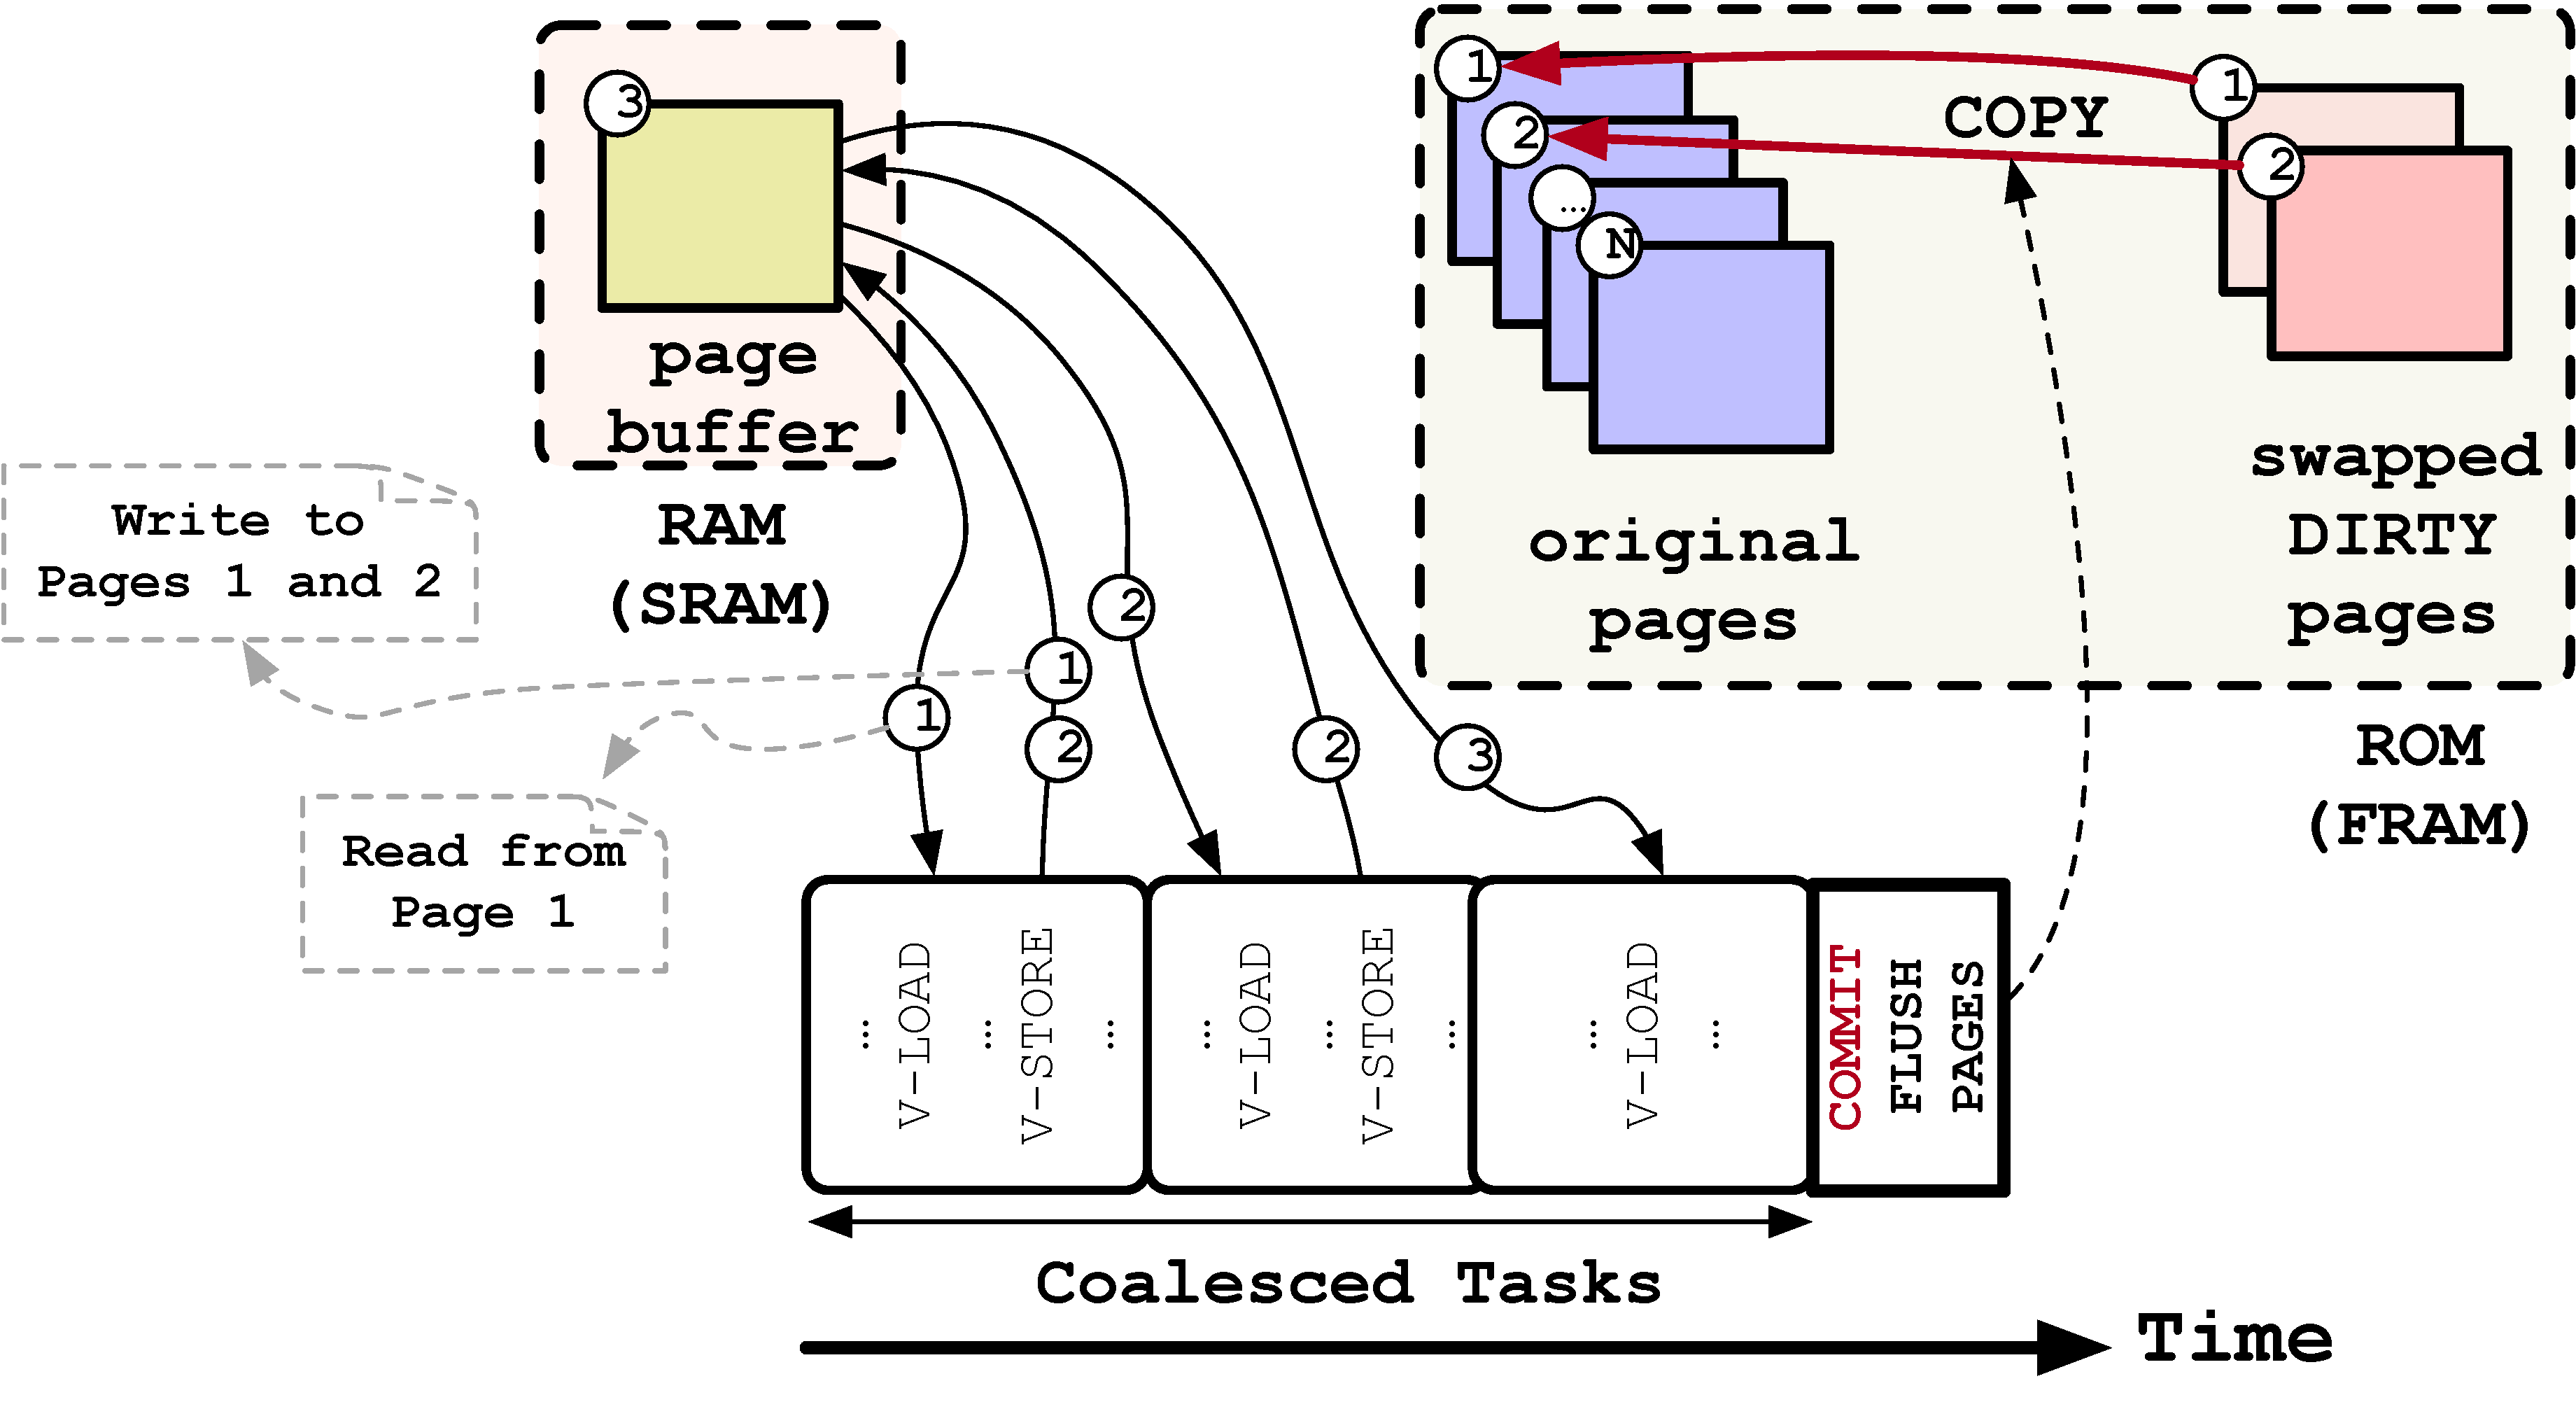
\includegraphics[width=\textwidth]{figures/graffle/paging.pdf}
	\caption{Illustration of \sys page tags mechanism.}
	\label{figure:coala_page_tags}
\end{figure}

We note that in order to obtain unique page tags, some alignment requirements have to be met. First, the page size $S$ has to be the power of two. Moreover, pages in non-volatile memory have to be aligned by $S$. Note that, by aligning pages by $2^n$, the alignment is also valid for all sizes $2^x$, where $x \leq n$.

\noindent \textbf{DMA Page Fault and Page Swap.} When a page is not found in RAM, it is fetched from FRAM. \todo{More explanation required here}{Carlo}

\subsection{\sys Scheduling and Committing}

\noindent \textbf{Target Budget Initialization.} Upon a reboot, the target budget (or target coalesced task size) has to be updated depending on the coalescing strategy. \todo{expand text}{Carlo}

\noindent \textbf{Coalescing State Recall.} The last (coalesced) task has to be recalled. More specifically, the function pointer of the last coalesced task has to be retrieved from a non-volatile memory, where is had been saved during the last successful commit. \todo{expand text}{Carlo}

\noindent \textbf{Partial Execution Restoration.} In case there is a valid partial execution checkpoint, the program has to resume from there \todo{expand text}{Carlo}

\noindent \textbf{Coalesced Scheduling.} \todo{expand text}{Carlo}

\noindent \textbf{Intermediate Commit and Ultimate Commit.} When a coalesced task is successfully run to completion, all the dirty pages in SRAM have to be persistently saved to a non-volatile memory. Since last version, no major changes were made to the intermediate commit (SRAM to shadow buffer), but an optimization was applied to the ultimate commit (shadow buffer to store buffer). Store buffer and shadow buffer used to be physically separated in memory. Now, the role of a block of memory (i.e. a page) is interchangeable, meaning that, during the ultimate commit, the shadow buffer pages that were written during the previous commit phase become store buffer pages, and their relative store buffer pages become shadow buffer pages. A page’s role is retrieved using an indirection table, i.e. an array that holds a zero for all the pages whose store buffer resides in the lower memory block, and a one for all the pages whose store buffer is located in the upper memory block. This allows for a lighter commit process, since fewer page moves are performed.

\begin{wrapfigure}{t!}{0.5\textwidth}
	\centering
	%\includegraphics[width=0.5\columnwidth]{figures/graffle/commits-illustration.pdf}
	\caption{Intermediate commit and ultimate commit Illustration \todo{to be drawn}{sinan}}
	\label{fig:intermediate_ultimate-commit}
\end{wrapfigure}

\noindent \textbf{Target Budget Update.} Before starting a new coalesced task, the target budget (or target coalesced task size) has to be updated depending on the coalescing strategy. \todo{expand text}{Carlo}

\todo{API of the partial commit needs to be explained as well}{Carlo}